\section{Uživatelské rozhraní}
Další nedílnou součástí procesu návrhu webové aplikace je tvorba wireframe. Wireframe představuje vizuální schéma, které zachycuje základní strukturu webu, rozložení jednotlivých prvků, jejich funkce a vzájemné vztahy. Slouží jako nákres či kostra aplikace, díky níž je možné si lépe představit způsob navigace a celkovou kompozici jednotlivých stránek. V této fázi se neklade důraz na grafické zpracování, ale spíše na funkčnost a logické uspořádání prvků. Z tohoto důvodu se wireframe zpravidla vytváří v jednoduché podobě, často pouze v odstínech šedi. \cite{wireframing}

\subsection{Hlavní stránka}
Hlavní stránka aplikace, označovaná jako dashboard, slouží jako úvodní přehledový panel, který uživateli poskytuje základní informace o jeho aktivitě. Je koncipována tak, aby uživateli umožnila rychlý přístup k nejdůležitějším údajům a zároveň zachovala přehlednou a jednotnou strukturu. Návrh rozložení této stránky je znázorněn na obrázku \ref{figure:wireframes-dashboard}.

V horní části stránky se nachází hlavička, která je shodná pro všechny části systému a zajišťuje snadnou orientaci napříč celou aplikací. Obsahuje logo aplikace, navigační menu umožňující přechod mezi jednotlivými stránkami a také ovládací prvky pro zobrazení profilu nebo odhlášení z aplikace.

Obsahová část dashboardu se zaměřuje na prezentaci statistických dat vztahujících se ke zvolenému časovému období. Uživatel zde může přehledně sledovat své aktivity a výkonnost prostřednictvím grafických vizualizací, které zobrazují rozložení aktivity vývojáře v čase nebo v rámci jednotlivých kategorií.

\begin{figure}[ht]
    \caption{Návrh hlavní obrazovky systému}
    \label{figure:wireframes-dashboard}
    \centering
    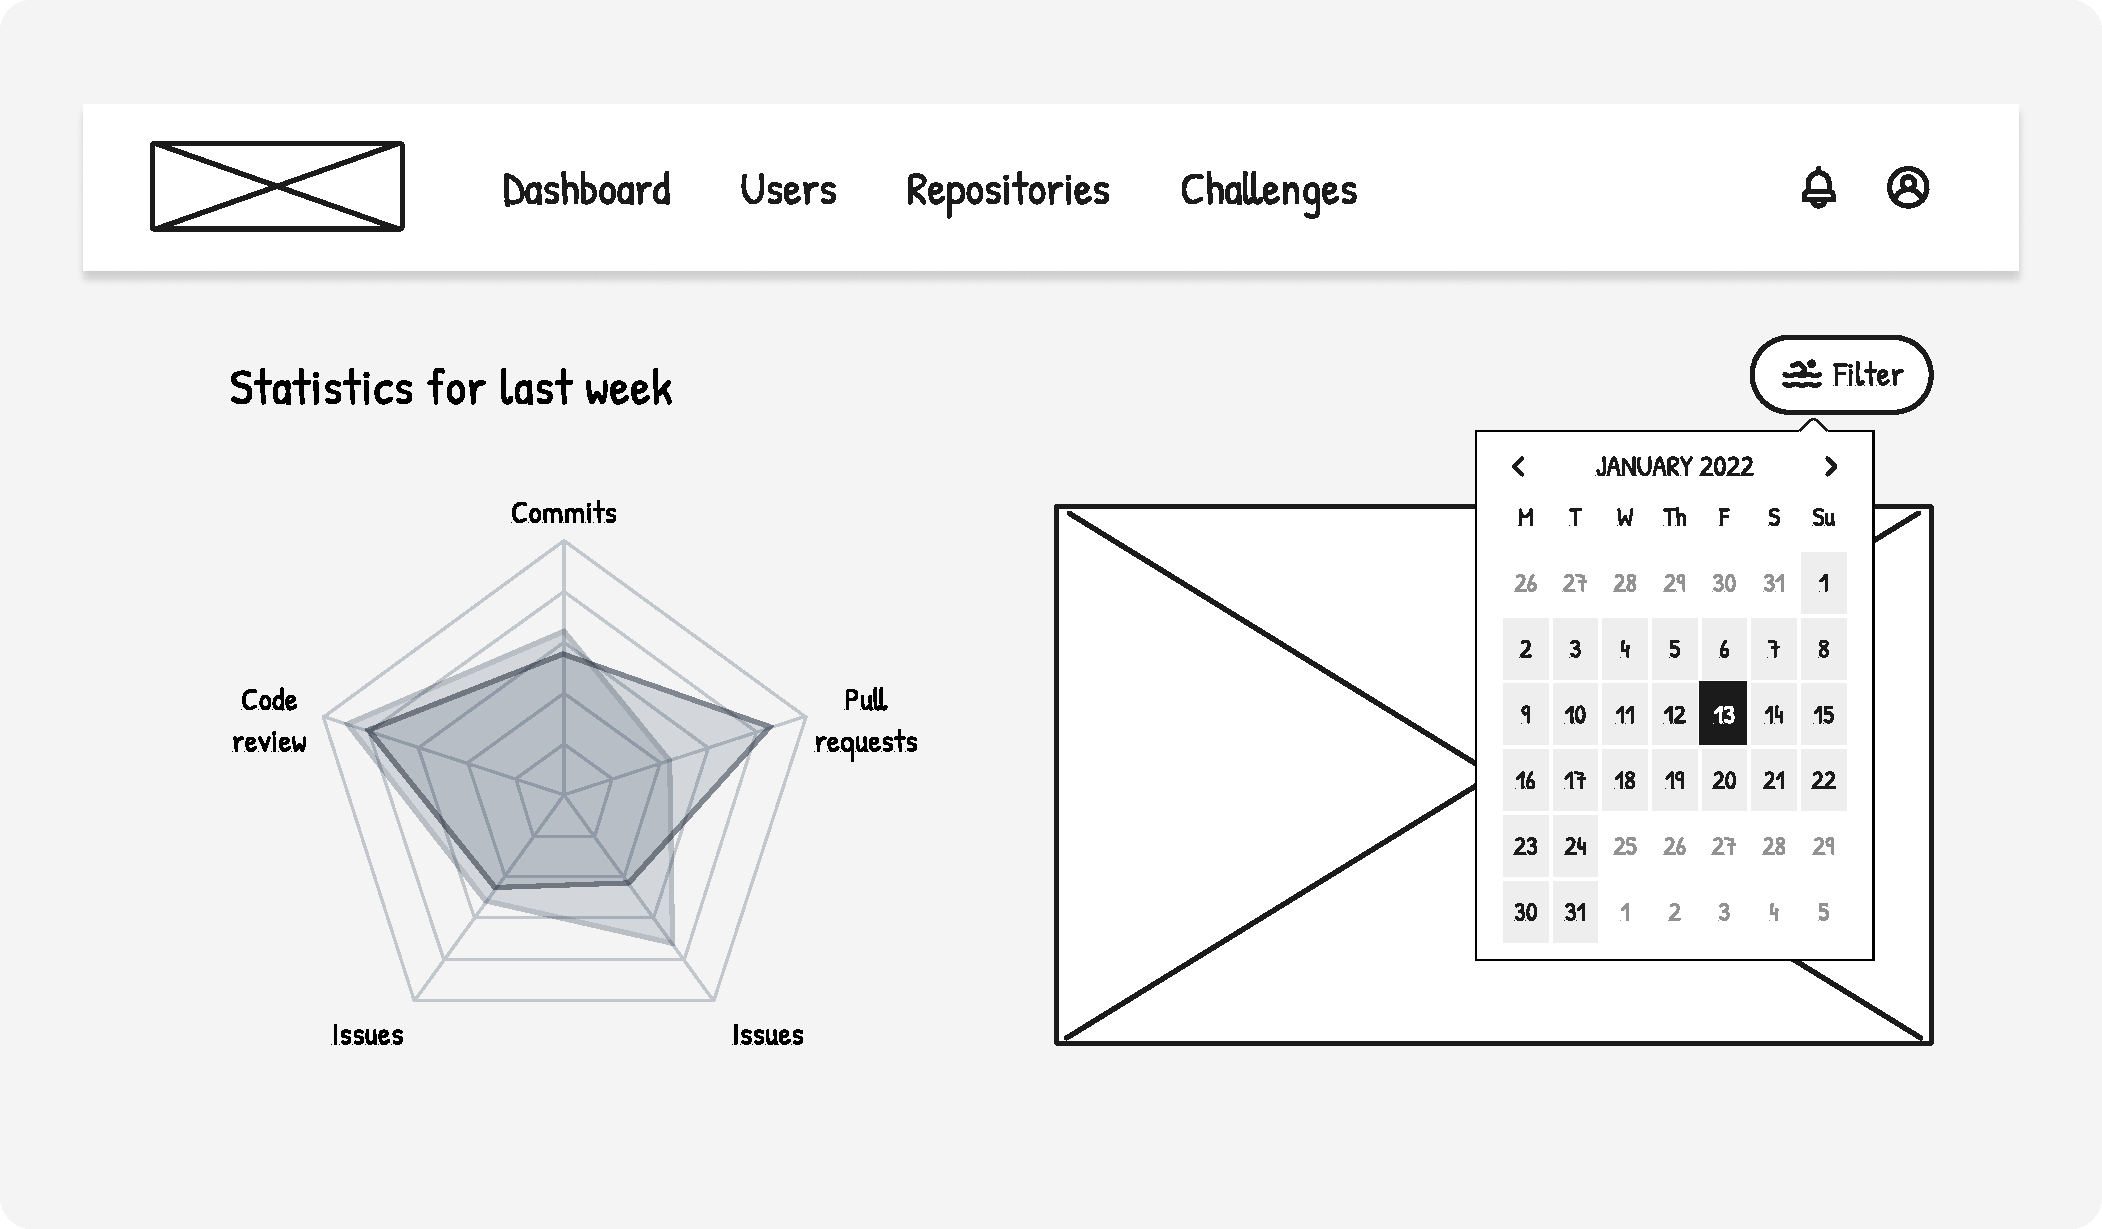
\includegraphics[width=0.98\linewidth]{images/wireframes/dashboard.pdf}
\end{figure}

\subsection{Tabulkové přehledy}
Vytvářená aplikace bude obsahovat více pohledů s tabulkovými přehledy. Návrh jednoho z těchto pohledů je znázorněn na obrázku \ref{figure:wireframes-user-index}, který představuje seznam uživatelů aplikace. Každý řádek tabulky zobrazuje základní informace o daném uživateli a nabízí možnost jeho úpravy nebo odstranění. Seznam podporuje stránkování a umožňuje upravit počet zobrazovaných položek na~stránku.

\begin{figure}[ht]
    \caption{Návrh obrazovky s přehledem uživatelů}
    \label{figure:wireframes-user-index}
    \centering
    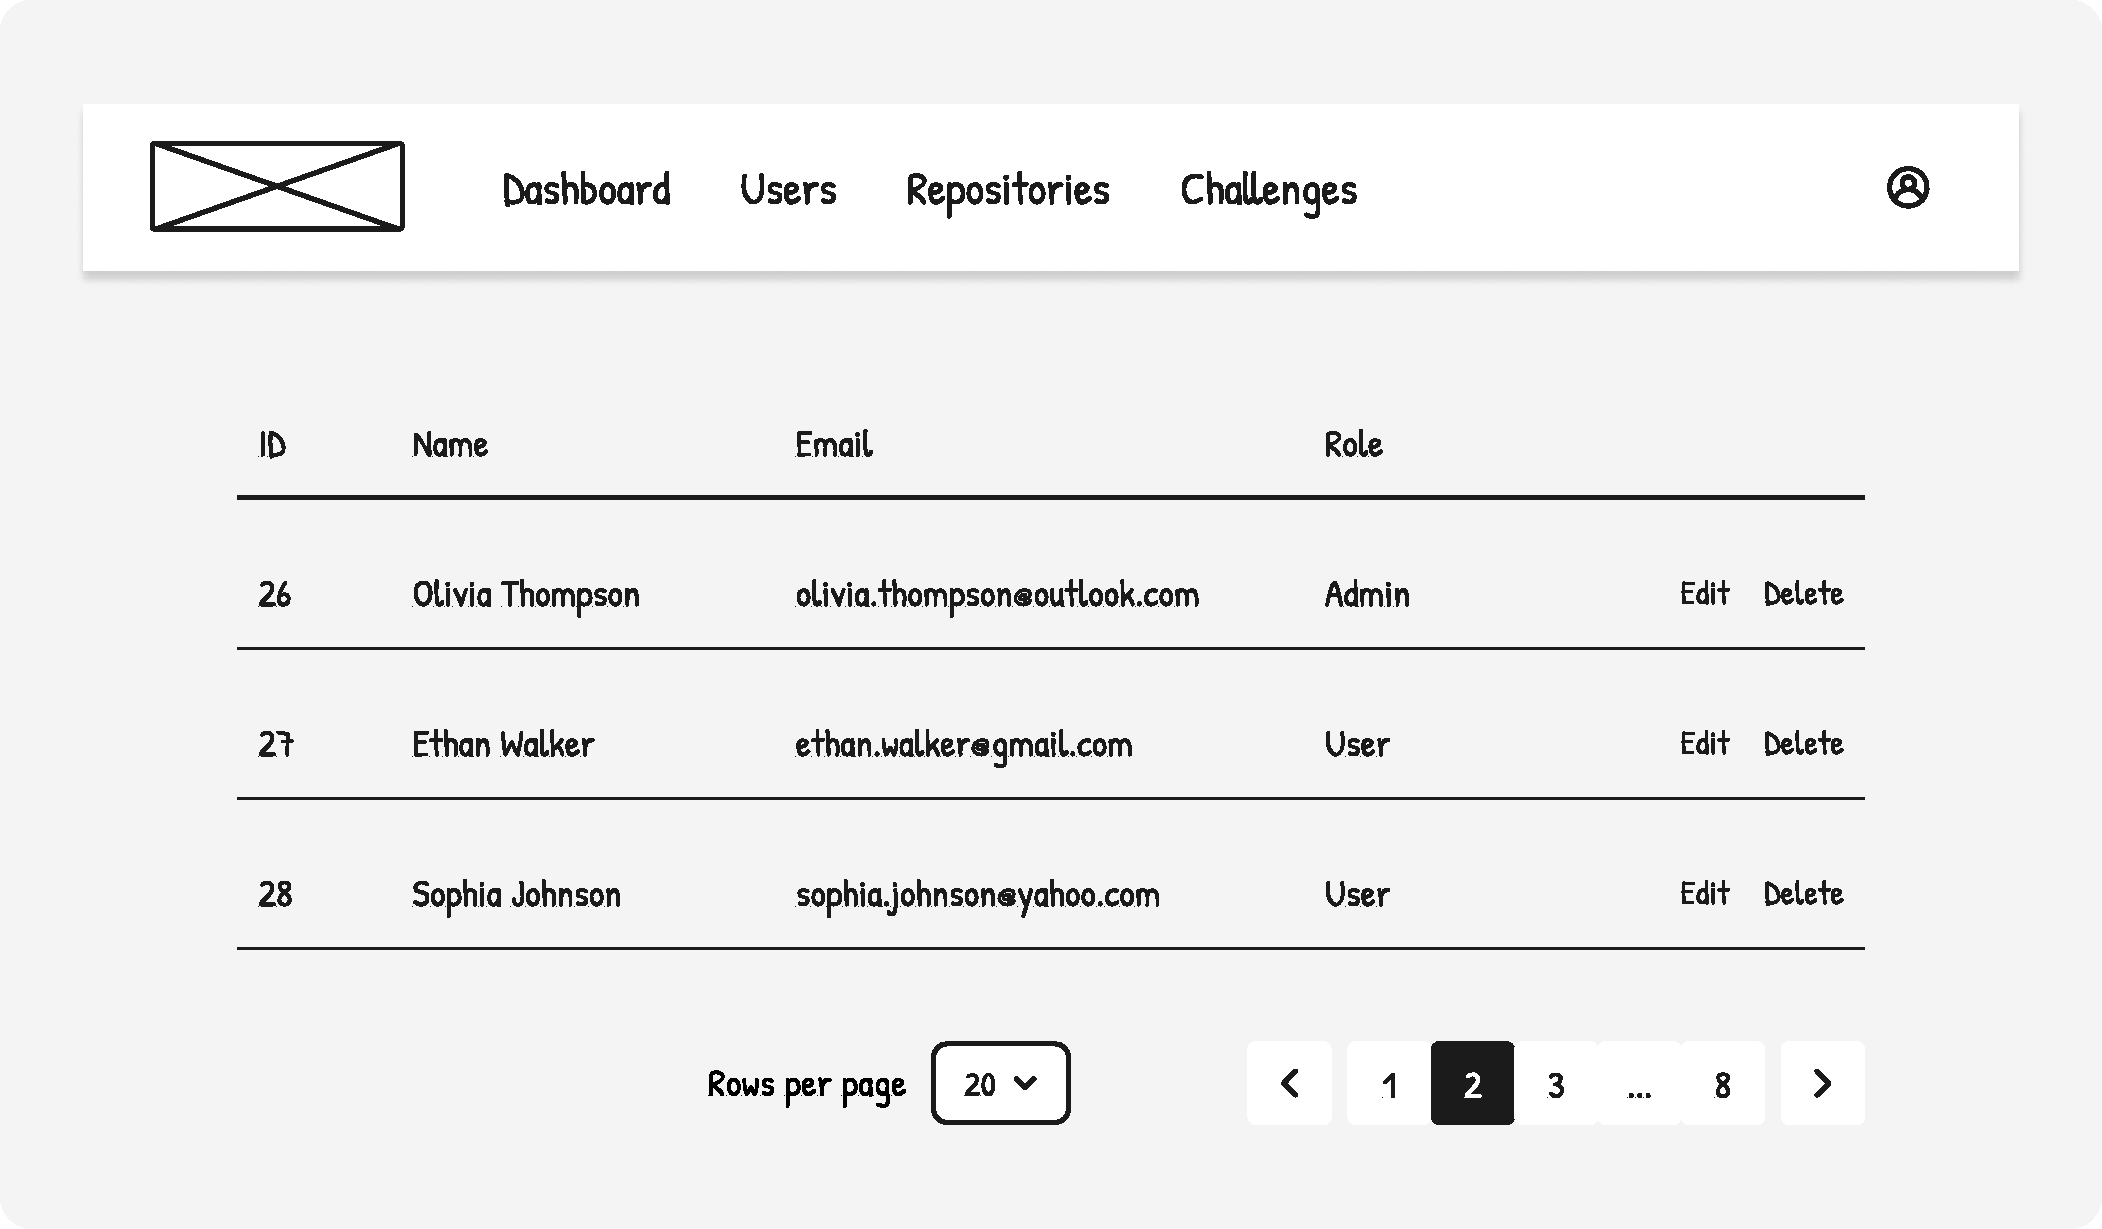
\includegraphics[width=0.98\linewidth]{images/wireframes/user-index.pdf}
\end{figure}
